\documentclass[a4paper, 10 pt, conference]{IEEEconf}
%\documentclass[a4paper, 10pt, conference]{ieeeconf}      % Use this line for a4 paper

\IEEEoverridecommandlockouts                              % This command is only needed if 
                                                          % you want to use the \thanks command

\overrideIEEEmargins  
%\usepackage[tmargin=2cm,lmargin=2cm,rmargin=2cm,bmargin=2.5cm]{geometry}
\usepackage[utf8]{inputenc}
\usepackage{cite}
\usepackage{graphicx} 
\usepackage{amsmath}
\usepackage{siunitx}
\usepackage{multirow}
%\usepackage{appendix}
\usepackage{comment} 
\usepackage{authblk}
\usepackage{algorithmicx}
%\usepackage{algorithm}% http://ctan.org/pkg/algorithm
\usepackage[ruled,linesnumbered]{algorithm2e}% http://ctan.org/pkg/algorithmicx
%\usepackage{caption}
%\usepackage{subcaption}
\usepackage[table]{xcolor}
\usepackage{lettrine}
\usepackage{url}
\usepackage{authblk}
\usepackage{amsfonts}
\usepackage{bm}
\let\proof\relax
\let\endproof\relax
\usepackage{amsthm}
\usepackage[english]{babel}
\usepackage{amssymb}

\newtheorem{theorem}{Theorem}
\newtheorem{lemma}[theorem]{Lemma}
\newtheorem{proposition}[theorem]{Proposition}
\newtheorem{corollary}[theorem]{Corollary}
\newtheorem{assumption}{Assumption}

\allowdisplaybreaks[4]
\newcommand\mcedit[1]{\textcolor{black}{#1}}
\newcommand\mdsedit[1]{\textcolor{black}{#1}}
\newcommand\mccheck[1]{\textcolor{black}{#1}}
\newcommand\mbedit[1]{\textcolor{black}{#1}}

\def\RR{\mathbb{R}}
\def\NN{\mathbb{N}}

\def\A{\mathcal{A}}
\def\B{\mathcal{B}}
\def\G{\mathcal{G}}
\def\S{\mathcal{S}}
\def\V{\mathcal{V}}
\def\U{\mathcal{U}}
\def\X{\mathcal{X}}

\def\Co{\mathrm{Co}}
\def\tr{\mathrm{tr}}
\def\bgamma{\boldsymbol{\gamma}}
\def\bc{{\bf c}}
\def\bS{\boldsymbol{\mathcal{S}}}


\title{\LARGE \bf
Difference of convex functions in robust tube MPC}


\author{Martin Doff-Sotta$^\star$
and
Mark Cannon$^\star$
\thanks{$^{\star}$Department of Engineering Science, University of Oxford, OX1 3PJ, UK
{\tt\small \{martin.doff-sotta,mark.cannon\}@eng.ox.ac.uk}}%
}%

\begin{document}

\maketitle
%\thispagestyle{empty}
\pagestyle{plain}

\begin{abstract}
We propose a  robust tube-based Model Predictive Control (MPC) paradigm for nonlinear systems whose dynamics can be expressed as a difference of convex functions. 
%
The approach exploits the convexity properties of the system model to derive convex conditions that govern the evolution of robust tubes bounding predicted trajectories. 
%
These tubes allow an upper bound on a performance cost to be minimised subject to state and control constraints as a convex program, the solution of which can be used to update an estimate of the optimal state and control trajectories. 
%
This process is the basis of an iteration that solves a sequence of convex programs at each discrete time step. 
%
We show that the algorithm is recursively feasible, converges asymptotically to a fixed point of the iteration and ensures closed loop stability.
%
The algorithm can be terminated after any number of iterations without affecting stability or constraint satisfaction.
%
A case study is presented to illustrate an application of the algorithm. 
%
% We propose DC-TMPC a tube-based Model Predictive Control (MPC) paradigm for nonlinear systems whose dynamics can be expressed as a difference of convex functions. The approach relies on successively perturbing the system predicted trajectories and bounding the linearisation error by exploiting convexity of the system dynamics. The linearisation error is then treated as a disturbance of the perturbed system to construct robust tubes containing the predicted trajectories, enabling the robust nonlinear MPC optimisation to be performed in  real time as a sequence of convex optimisation programs. Convergence, recursive feasibility and stability of the proposed approach are demonstrated. A case study involving a coupled tank problem is presented to illustrate an application of the algorithm. 
%
\\
\noindent\textbf{Keywords:}
nonlinear MPC, robust receding horizon control, convex optimisation, difference of convex functions
\end{abstract}

\section{Introduction}
\noindent Robust model predictive control (MPC) algorithms aim to provide performance and closed-loop stability guarantees in the presence of model or measurement uncertainty, while ensuring constraint satisfaction and  tractable computation. 
%
Robust tube MPC refers to a collection of strategies that  
%
%These methods are based on the idea that 
use information on the uncertainty affecting predictions to bound the future trajectories of the system~\cite{kouvaritakis,rawling}.
%
%Tube-based MPC is a specialised robust MPC technique that conveniently relies on a parameterisation of the uncertainty sets in terms of a tube in which the system trajectories are guaranteed to remain. 
A tube consists of a sequence of sets containing predicted future system trajectories for all realisations of uncertainty. %Robust stabilisation of the system trajectory $x_k$ into a tube is made possible via a two-degree-of-freedom controller $u_k = c_k + \kappa(x_k, x^0_k)$. On the one hand, a feedforward control sequence $c_k$ is computed to stabilise the system around a nominal trajectory $x^0_k$. It is derived online by minimisation of an optimisation cost for the nominal system subject to tightened constraint sets that account for the presence of bounded disturbances. On the other hand, a state feedback controller $\kappa(x_k, x^0_k)$ is designed to steer the system inside the uncertainty sets. 
%

Tube-based MPC has been successfully applied to robust stabilisation problems for linear systems \cite{gossner1997stable, schuurmans2000robust, lee1999constrained, chisci2001systems, goulart, langson2004robust, rakovic2012homothetic, mayne2005robust}. %See \cite{kouvaritakis} or \cite{rawling} for a modern treatment.
%
The application of tube-based MPC to nonlinear systems poses a series of challenges: in particular online solution of nonconvex optimisation problems, safe approximation of uncertainty sets for states described by nonlinear dynamics, and the computational complexity associated with searching for  general nonlinear feedback policies. An early implementation of robust MPC to nonlinear uncertain systems was proposed in \cite{mayne2007tube} with a tube MPC framework that relies on the concept of constraint tightening as introduced in \cite{michalska1993robust}. %The control law is computed using two successive MPC controllers: on the one hand, the central line of the tube is obtained by minimising a nominal cost subject to nonlinear dynamics and tightened constraint sets, while on the other hand, an ancillary MPC law is used to reject the disturbances acting on the system and maintain the trajectory within sets of known size centred along the tube line. Computation of the tightened constraint sets is more difficult in the nonlinear case because the system describing the evolution of the error is no longer autonomous and the error is thus less easily bounded \cite{rawling}.

In some cases the special structure of the system dynamics can be exploited to good advantage to define a nonlinear tube MPC framework. In \cite{rakovic2006simple}, a method is proposed for nonlinear systems with input-matched nonlinearities and nonlinear processes that take the form of piecewise affine maps. Feedback linearisation is used to cancel nonlinearities and a two-degree-of-freedom linear control law stabilises the system trajectory in a tube formed by robustly invariant sets. A method is proposed in \cite{yu2013tube} for constructing robust invariant sets for a class of Lipschitz nonlinear systems, relying on the computation of a quadratic Lyapunov function and an associated state feedback controller. In practice, this approach is limited since finding a global Lipschitz constant may result in a conservative controller with poor performance. Nonlinear system dynamics with a differential flatness property can also be advantageously reformulated to define a tube-based receding-horizon controller as in \cite{petkar2016robust}.

A common strategy in nonlinear tube-based MPC is to treat the nonlinearity in the dynamics as a bounded disturbance \cite{lee2002constrained, althoff2008reachability, cannon2009successive, mark}. In \cite{mark}, successive linear approximations around predicted trajectories are used to obtain a MPC law for nonlinear systems with differentiable dynamics. The proposed algorithm uses bounds on linearisation errors to construct an ellipsoidal tube and an associated control law. The controller achieves rejection of the linearisation error and stabilisation of the nonlinear system, %within a tube formed with  ellipsoidal sets. 
and approach has guarantees of recursive feasibility and asymptotic stability.

%Although in principle computationally tractable, 
These strategies rely for robustness on bounds on linearisation errors, which are either computed using fixed prior bounds on predicted future states, and are therefore conservative, or otherwise may present computational difficulties. In this work we show that tighter bounds can be obtained under certain convexity assumptions. We consider systems that can be expressed as a difference of convex functions~\cite{horst99:dcprog,hartman59:dcfun}. 
The convexity properties of these systems considerably simplify the problem of determining bounds on model states that are suitable for defining predicted state tubes. We derive convex conditions for the evolution of tubes bounding perturbations on future predicted trajectories. Analogously to successive linearisation approaches, these conditions form the basis of an iteration that solves a sequence of convex programs to minimise a bound on predicted cost subject to robust constraint satisfaction. The iteration is recursively feasible and convergent, and the resulting MPC algorithm is asymptotically stabilising. 
%A convex nonlinear function developed as a Taylor series truncated to the first order term has a convex  linearisation error.  For convex  linearisation errors defined on compact sets, the maximum occurs at the boundary of the domain, and the minimum is zero, which allows to construct non-conservative bounds for the error. If the error is treated as a disturbance of the perturbed dynamics, the tube-based MPC formalism can be applied efficiently to robustly stabilise the nonlinear system in real time. 

The paper is organised as follows. 
%After a quick theoretical reminder on notations and 
Tube MPC based on successive linearisation is discussed in Section  \ref{sec:TMPC}, then Section \ref{sec:theory} presents the proposed new MPC approach (DC-TMPC) based on the difference of convex functions. The convergence, stability and feasibility properties of the algorithm are discussed in Section  \ref{sec:convergence}. To illustrate the approach, we describe its application to the problem of regulating fluid in a pair of coupled tanks in Section \ref{sec:case}. 

\textit{Notation:}
%\label{sec:notations}
%$\mathbb{N}_p$ denotes $\{0,\ldots,n\}$.
The value of a variable $x\in \RR^{n_{x}}$ at the $n$th discrete time step is denoted $x[n]$, and a sequence predicted at discrete time $n$ is denoted %$\{x_{k}\}_{k=0}^{N-1}=\{ x_{k}, \, k\in\NN_{N-1}\}$, 
$\{x_{k}\}_{k=0}^{N-1}=\{ x_{0} , \ldots, x_{N-1}\}$, 
where $x_{k}$ is the predicted value of $x[n+k]$.
%
A symmetric matrix $P\in\RR^{q\times q}$ is positive definite (resp.~semidefinite)  if ${P\succ 0}$ ($P\succeq 0$), and the weighted Euclidean norm is denoted $\lVert x\rVert_P := (x^\top P x)^{1/2}$.
%
For $K\in\RR^{p\times q}$ and sets $\A,\B\subset\RR^{q}$ we denote $\A \oplus \B := \{a + b : a \in \A, \, b \in \B\}$, $ K \A := \{K a : a \in \A \}$, and $\lVert \A \rVert_P = \max_{a\in\A} \lVert a \rVert_P$.
%
The $k$th element of a function $f:\RR^p\to\RR^q$ is denoted $[f]_k$ and $f$ is called a DC function (or simply DC) if $f = g - h$, where $g,h:\RR^p\to\RR^q$ are such that $[g]_k,[h]_k$ are convex functions for $k=1,\ldots,q$.

%  with convex entries.
% that is $k$ times continuously differentiable functions is denoted $C^k$ and 
% We write $ C^k$ if $f$ is $k$ times continuously differentiable, and $f:\RR^n\to\RR^n$ is 

%The set subtraction is defined by $\S_1 \ominus \S_2 :=  \{x \in \RR^{n_{x}}: \{x\} \oplus  \S_1 \subseteq \S_2\}$. 
%$\{x\}$ denotes the set formed by a single point $x$, so $\{x\} \oplus \mathcal{A} = \{x + a : a \in \mathcal{A} \}$. 



\section{Successive linearisation tube MPC}
\label{sec:TMPC}

Consider the following discrete-time dynamical system 
%
\begin{equation}
\label{eq:dyna}
x[n+1] = f(x[n], u[n]) .
\end{equation}
Here $x \in \X$, $u \in \U$ are state and control variables and $\X\subset\RR^{n_x}$, $\U\subset\RR^{n_u}$ are compact constraint sets. The goal is to regulate $(x[n],u[n])$ around a reference  $(x^r[n],u^r[n])$ (where ${x^r[n+1]} = f(x^r[n],u^r[n])$ and $(x^r[n],u^r[n])\in\X\times\U$), while minimising a quadratic cost. 
% subject to input and state constraints. 
%
To simplify presentation we discuss here the case of a constant reference $(x^r,u^r)$.

%Finding a nonlinear MPC controller for system \eqref{eq:dyna} in general is hard and can be intractable for large online problems. 
%
%One popular approach is, at each time step $n$, to successively 
Successive linearisation MPC addresses the optimal control problem to be solved online at each discrete time step by considering perturbations of previously computed predicted trajectories of the system.
%with dynamics described by an approximate linear model.
% 
%Under Assumption~\ref{assump:lin}, 
This approach repeatedly linearises the model~(\ref{eq:dyna}) around state and control trajectories, defined at time $n$ by ${\bf x}^\circ = \{x_k^\circ\}_{k=0}^N$, ${\bf u}^\circ=\{u_k^\circ\}_{k=0}^{N-1}$, with $x^\circ_0=x_0=x[n]$ and $x^\circ_{k+1} = f(x_k^\circ,u_k^\circ)$ for $k=0,\ldots,{N-1}$.
%over a horizon of $N$ steps. 
In~\cite{mark} the linearisation errors are treated as unknown bounded disturbances and a robustly stabilising two-degree of freedom controller is designed for the linearised dynamics by solving a sequence of convex optimisation problems.  

Defining the predicted state and control perturbations as $s_k = x_k - x^\circ_k$ and $v_k = {u_k-u^\circ_k}$ respectively, we construct a tube (a sequence of sets) $\bS = \{\S_k\}_{k=0}^N$ so that $s_k\in\S_k$ for all $k$.
%the predicted state and input perturbation tubes as the collection of sets $\S=\{\S_0, \ldots, \S_N\}$ and $\V=\{\V_0, \ldots, \V_{N-1}\}$. 
%
The perturbed state satisfies $s_0=0$ and
%
% \begin{equation}\label{eq:perturbed_state}
\[
s_{k+1} = A_k s_k + B_k v_k  + g_k, 
\]
% \end{equation}
% %
% \begin{align*}
% x_{k+1}^\circ + s_{k+1} &= f(x_k^\circ + s_k, u_k^\circ + v_k) 
% \\
% &= f(x_k^\circ, u_k^\circ) + A_k s_k + B_k v_k  + g_k, 
% \end{align*}
for $k= 0, \ldots, N-1$, where $A_k = \frac{\partial f}{\partial x}(x_k^\circ, u_k^\circ)$, $B_k = \frac{\partial f}{\partial u}(x_k^\circ, u_k^\circ)$, and $g_k$ is the remainder term in the first-order Taylor expansion of $f$ about $(x_k^\circ,u_k^\circ)$. For  the Jacobian linearisation to exist, the following assumption was implied

\begin{assumption}\label{assump:lin}
$f$ is differentiable on $\X\times\U$.
\end{assumption}

%
The predicted control perturbation sequence is parameterised with a feedforward term $c_k$ and a linear feedback term $K_k s_k$, for $ k = 0,\ldots, N-1$,
\begin{equation}
\label{eq:input}
v_k = c_k + K_k s_k.
\end{equation}
Defining $\Phi_k = A_k +  B_k K_k$ and given bounds $g_k\in\G_k$ on linearisation errors, the sets $\S_k$ defining the tube cross-sections therefore satisfy $\S_0=\{0\}$ and, for $k= 0, \ldots, {N-1}$,
\begin{equation}\label{eq:tube0}
\S_{k+1} \supseteq \Phi_k \S_k \oplus \{ B_k   c_k\} \oplus \G_k.
\end{equation}
The tube $\bS$ and the feedforward sequence $\bc=\{c_k\}_{k=0}^{N-1}$ are variables in an optimal tracking control problem with cost
%with state and input constraints and with finite horizon quadratic cost 
\begin{align}
& J(\bc,\bS,{\bf x}^\circ,{\bf u}^\circ) =  \sum_{k = 0}^{N-1}\bigl[\lVert \{x_k^\circ - x^r\}\oplus \S_k \rVert_Q^2  
\nonumber \\
&+ \lVert \{u_k^\circ + c_k- u^r\} \oplus K_k\S_k \rVert_R^2\bigr]
+ \lVert \{x_N^\circ - x^r\} \oplus \S_N \rVert_{\hat{Q}}^2
\label{eq:cost}
\end{align}
where $Q \succ 0$, $R \succ 0$. The terminal weighting matrix $\hat{Q} \succ 0$ is chosen so that, for all $x\in\hat{\X}$, 
\begin{multline}\label{eq:Q_N}
\lVert x-x^r\rVert_{\hat{Q}}^2 \geq 
\lVert f(x,\hat{K}(x - x^r)+u^r) - x^r\rVert_{\hat{Q}}^2 
\\
+ \lVert x - x^r \rVert_Q^2
+ \lVert \hat{K}( x - x^r) \rVert_Q^2 ,
\end{multline}
where the terminal set $\hat{\X}$ and feedback gain $\hat{K}$ satisfy
%$\hat{\X}\subseteq\X$ and 
%$\hat{K}\hat{\X}\oplus\{u^r-Kx^r\}\subseteq \U$.
\begin{equation}\label{eq:termset_feas}
\hat{\X}\subseteq\X, \quad 
\hat{K}\hat{\X}\oplus\{u^r-\hat{K} x^r\}\subseteq \U.
\end{equation}
The terminal set can be defined, for example, in terms of a scalar $\hat{\gamma}$:
\begin{equation}\label{eq:termset_def}
\hat{\X} = \{ x : \lVert x\rVert_{\hat{Q}}^2 \leq \hat{\gamma} \}
\end{equation}
The terminal parameters $\hat{K}$, $\hat{Q}$ and $\hat{\gamma}$ can be computed simultaneously offline by solving a convex optimisation problem (see the Appendix).
%
% \begin{align}
% \hat{\gamma} &\geq \max_{s_N} || x_N^\circ + s_N - x_N^r ||_{Q_N}^2 
% \nonumber\\
% &\geq \max_{s_N} || x_N^\circ + s_N - x_N^r ||_{Q}^2 
% + \max_{s_N} ||u_N - u_N^r||_{R}^2 
% \nonumber\\
% &\quad + \max_{s_N} || f(x_N^\circ + s_N, u_N - u_N^r) - x_{N+1}^r||_{Q_N}^2,  
% \label{eq:Q_N}
% \end{align}
The gains $\{K_k\}_{k=0}^{N-1}$ in equation \eqref{eq:input} can be computed, for example, using a dynamic programming recursion initialised with $P_N = \hat{Q}$, and, for $k=N-1, \dots , 0$, 
%
\begin{equation}\label{eq:dp}
\begin{aligned}
\Delta_k &= B_k^\top P_{k+1} B_k + R
\\
K_k &= -\Delta_k^{-1} B_k^\top P_{k+1} A_k
\\
P_k &= Q + A_k^\top P_{k+1} A_k - A_k^\top P_{k+1}B_k \Delta_k^{-1} B_k^\top P_{k+1} A_k
\end{aligned}
\end{equation}
%Alternatively $K_k=\hat{K}$ may be used for all $k$.
%. Note that the feedback term mitigates the effects of uncertainty in the model, namely the linearisation error $g_k$. 

The MPC optimisation at time $n$ is initialised with a feasible predicted trajectory $({\bf x}^\circ, {\bf u}^\circ)$ of (\ref{eq:dyna})
%such that $(x_k^\circ,u_k^\circ)\in\X\times\U$ for all $k$
%At each time step $n$, we obtain successive approximations of the trajectory 
and the following optimisation problem in variables $\bc$, $\bS$ %$\bgamma=\{\gamma_k\}_{k=0}^N$ 
is solved sequentially
\begin{equation}\label{eq:iteropt0}
\begin{alignedat}{2}
&  \min_{\bc,\bS} &  \ &   J(\bc,\bS,{\bf x}^\circ,{\bf u}^\circ) 
\ \text{subject to, $\forall k \in \{0, \ldots, N-1\}$,}
\\ 
% & & & \lVert \{x_k^\circ - x_k^r\} \!\oplus\! \S_k \rVert_Q^2 
% +  \lVert \{u_k^\circ \!+\! c_k - u_k^r\} \!\oplus\!  K_k \S_k \rVert_R^2  
% \leq\gamma_k
% \\
& & &
\Phi_k \S_k \oplus \{B_k c_k\} \oplus \G_k \subseteq \S_{k+1}
\\
& & & 
\{x_k^\circ\} \oplus \S_k \subseteq \X 
\\
& & &    \{u_k^\circ+c_k\} \oplus K_k \S_k \subseteq \U 
% \\
% &&& \hspace{40mm} \forall k \in \{0, \ldots, N-1\};
\\
& & &  \lVert \{ x_N^\circ - x^r\} \oplus \S_N \rVert_{\hat{Q}}^2 \leq \hat{\gamma}
% \\
% & & & \gamma_N \leq \hat{\gamma}
%& & &   \{x_N^\circ\} \oplus \S_N \in \{x_N^r\} \oplus \{x: \lVert x \rVert_{Q_N}^2 \leq \hat{\gamma}\},
\\
& & &    \S_0 = \{0\}.
\end{alignedat}
\end{equation}
%
The solution of (\ref{eq:iteropt0}) for $\bc$ is used to update $({\bf x}^\circ,{\bf u}^\circ)$ by setting%
%
\begin{subequations}\label{eq:iter1}%
\begin{alignat}{2}
s_0 &\gets 0, 
\\
\label{eq:iter2}
u^\circ_k &\gets u^\circ_k + c_k + K_k s_k, 
%\quad & \forall k &\in \{0, \ldots , N-1\}, 
\\
\label{eq:iter3}
s_{k+1} &\gets f(x^\circ_k, u^\circ_k) - x^\circ_{k+1}, 
%\quad & \forall k &\in \{0, \ldots , N-1\},
\\
\label{eq:iter4}
x^\circ_{k+1} &\gets f(x^\circ_k, u^\circ_k),  
% \quad & \forall k & \in \{0, \ldots , N-1\},
\end{alignat}
\end{subequations}
for $k = 0, \ldots , N-1$, and the process (\ref{eq:iteropt0})-(\ref{eq:iter1}) is repeated until $\lVert \bc \rVert^2 := \sum_{k=0}^{N-1}\lVert c_k\rVert^2$ has converged to a sufficiently small value or the maximum number of iterations is reached. 
%
The control law is then implemented as
\begin{equation}
\label{eq:step_update1}   
u[n] = u^\circ_{0}.
% \quad
% %\label{eq:step_update2}   
% x[n+1] = f(x[n], u[n]),
\end{equation}
%

%A new iteration is initialised at time $n$ using the solution computed at $n-1$ by setting 
At time $n+1$ we set $x^\circ_0 \gets  x[n+1]$ and initialise a new iteration with $({\bf x}^\circ,{\bf u}^\circ)$ defined, for $k=0,\ldots,N-1$, by
\begin{subequations}\label{eq:step_update3}
\begin{align}
u^\circ_{k} &\gets u^\circ_{k+1}, 
%, \, \forall k \in \{0, \ldots , N-2\}, 
\\
\label{eq:step_update4}
x^\circ_{k+1} &\gets  f(x^\circ_{k}, u^\circ_{k}), 
%, \, \forall k \in \{0, \ldots, N-2\},
\\
\label{eq:step_update5_}
 u^\circ_{N-1} &\gets \hat{K}(x^\circ_{N-1} - x^r) + u^r,
\\
\label{eq:step_update5}
x^\circ_{N} &\gets  f(x^\circ_{N-1}, u^\circ_{N-1}).
\end{align}
\end{subequations}
These definitions ensure recursive feasibility of the scheme. In addition, the optimal value of $J(\bc,\bS,{\bf x}^\circ,{\bf u}^\circ)$ is non-increasing at successive iterations, implying that the iteration converges asymptotically: $\bc \to 0$ and $\bS\to\{\{0\},\ldots,\{0\}\}$, and also non-increasing at successive time steps $n=0,1,\ldots$, implying that $(x,u)= (x^r,u^r)$ is an asymptotically stable equilibrium (see e.g.~\cite{mark}, Theorems 7 and 8 for details).

% of the system lie within tubes arising from the successive predicted trajectories ${\bf x}^\circ$ and whose cross sections form robustly invariant sets whose size is adjusted by the feedback term $K_k s_k$. 

Despite its attractive theoretical properties, the successive linearisation approach relies on bounds on the linearisation error $\G_k$, which are difficult to compute in general and might result in overly conservative bounds if no further assumptions are made on $f$. Moreover, the algorithm outlined in this section does not ensure convergence to a solution that satisfies the first order optimality conditions for the problem of minimizing $\sum_{k=0}^{N-1} [\|x_k-x^r\|_Q^2 + \|u_k-u^r\|_R^2] + \|x_N-x^r\|_{\hat{Q}}^2$ subject to $x_{k+1}=f(x_k,u_k)$, $x_k\in\X$ and $u_k\in\U$ since $\G_k$ may not be tight.
To overcome these problems, we propose a method for systems~(\ref{eq:dyna}) in which $f$ is a DC function to obtain tight bounds on linearisation errors.


\section{Successive convex programming tube MPC for DC systems}
%\section{Nonlinear tube-based model predictive control for DC systems}
\label{sec:theory}

%Returning to the model~(\ref{eq:dyna}), 
To derive a control algorithm with reduced computation and improved performance, we strengthen our assumptions
%Assumption~\ref{assump:lin} 
on model~(\ref{eq:dyna}) as follows.

\begin{assumption}\label{assump:dc}
$f$ is DC on $\X\times\U$ and $\X,\U$ are convex sets.
\end{assumption}

Under Assumption~\ref{assump:dc} the model~(\ref{eq:dyna}) can be expressed
%
\begin{align}
\label{eq:DC}
x[n+1] =  f_1(x[n], u[n]) -  f_2(x[n], u[n]),  
\end{align}
where each component of the vector-valued functions $f_1, f_2$ is a convex function. 
%
Note that~(\ref{eq:DC}) includes systems in which $f$ in (\ref{eq:dyna}) is either convex or concave. 
%
More generally, any twice continuously differentiable function is DC and any continuous function can be approximated arbitrarily closely by a DC function on a compact convex set~\cite{horst99:dcprog,hartman59:dcfun}, which extends considerably the scope of the present method.

Given a predicted trajectory $({\bf x}^\circ, {\bf u}^\circ)$ of (\ref{eq:dyna}), the perturbed variables $s_k = x_k - x_k^\circ$, $v_k = u_k - u_k^\circ$ are governed by $s_0=0$ and, for $k=0,\ldots,N-1$,
%
\begin{equation*}
s_{k+1} =A_{1, k} s_k + B_{1, k} v_k + g_{1, k} - (A_{2, k} s_k + B_{2, k} v_k + g_{2, k}), 
\end{equation*}
where for $i=1,2$, $A_{i, k} = \frac{\partial f_i}{\partial x}(x_k^\circ, u_k^\circ)$, $B_{i, k} = \frac{\partial f_i}{\partial u}(x_k^\circ, u_k^\circ)$,
%
% \[A_{1, k} = \frac{\partial f_1}{\partial x}\Bigr|_{\substack{(x_k^\circ, u_k^\circ, 0)}}, \quad  A_{2, k} = \frac{\partial f_2}{\partial x}\Bigr|_{\substack{(x_k^\circ, u_k^\circ, 0)}}, 
% \]
% \[B_{1, k} = \frac{\partial f_1}{\partial u}\Bigr|_{\substack{(x_k^\circ, u_k^\circ, 0)}}, \quad B_{2, k} = \frac{\partial f_2}{\partial u}\Bigr|_{\substack{(x_k^\circ, u_k^\circ, 0)}}, 
% \] 
% \[D_{1, k} = \frac{\partial f_1}{\partial w}\Bigr|_{\substack{(x_k^\circ, u_k^\circ, 0)}}, \quad D_{2, k} = \frac{\partial f_2}{\partial w}\Bigr|_{\substack{(x_k^\circ, u_k^\circ, 0)}}, 
% \]
%
and $g_{i,k} $ represents the error in the Jacobian linear approximation of $f_i$ around $(x_k^\circ,u_k^\circ)$.
%
Using the control law \eqref{eq:input}, defining
$\Phi_{i, k}=A_{i, k}+B_{i, k} K_{k}$, $i =1, 2$, 
% the perturbed system becomes
% \[%\begin{align*}
% s_{k+1} =\Phi_{1, k} s_k + B_{1, k} c_k + g_{1, k} - (\Phi_{2, k} s_k + B_{2, k} c_k +  g_{2, k}) .
% \]%\end{align*}
and assuming bounds $g_{i, k} \in \G_{i, k}$, $i=1,2$, we obtain a set of constraints to be satisfied by the tube cross-sections $\S_k$ containing $s_k$:
%are obtain the tube constraint analogous to~(\ref{eq:tube0}) as
%
\begin{equation}
\label{eq:tube}
\S_{k+1} \supseteq (\Phi_{1, k} - \Phi_{2, k})\S_k \oplus \{ (B_{1, k} - B_{2, k}) c_k\} \oplus \G_{1, k} \oplus -\G_{2, k}. 
\end{equation}

We now characterise the sets $\S_{k}$ and $\G_{i, k}$ to obtain a workable formulation of these constraints.
%
Various parameterisations of the sets $\S_k$ are possible: polytopic,  ellipsoidal, homothetic (e.g.~\cite{kouvaritakis}). In this work, for simplicity, we define a polytopic tube cross-section in terms of elementwise bounds:
%
\[
\S_k = \{ (s_{1}, \ldots, s_{n_x})\!\in\!\RR^{n_x} : \underline{s}_{k, j} \!\leq\! s_{j} \!\leq\! \bar{s}_{k, j},  \, j = 1, \ldots, n_x \} .
\]
Considering $g_{1,k}$, $g_{2,k}$ as functions of $s_k$ and $c_k$:
\[%\begin{multline}
g_{i,k} \!=\! 
f_i(x^\circ_k + s_{k}, \! u^\circ_k + v_k) - f_i(x^\circ_k, \! u^\circ_k) - \Phi_{i, k} s_k - B_{i, k} c_k,  
%\label{eq:error1}
\]%\end{multline}
the convexity of $f_i(x,u)$ for $(x,u)\in\X\times\U$ implies that $g_{i,k}(s,c)$ 
is convex for all $(s,c)$ such that $(x^\circ+s,u^\circ+Ks+c)$ lies in $\X\times\U$. It follows that, for $i=1,2$,
%is a Jacobian linearisation error and $g_{i}(x^\circ,u^\circ,s,v)$ 
%
\begin{align*}
& \min_{\substack{s_k \in \S_k}} g_{i,k}(s_k,c_k) = 0,
\\
& \max_{\substack{s_k \in \S_k}} g_{i,k}(s_k,c_k) = \max_{\substack{s \in \V(\S_k)}} g_{i,k}(s,c_k), 
\end{align*}
%
where $\V(\S_k)$ denotes the set of vertices of $\S_k$. The tube constraint \eqref{eq:tube} is therefore ensured by the convex inequalities
%
\begin{align*}
\underline{s}_{k+1} &\leq \! \min_{\substack{s \in \V(\S_k})} \! \{(\Phi_{1, k}\!-\!\Phi_{2, k}) s + (B_{1, k}\!-\!B_{2, k}) c_k - g_{2,k}(s)\},
\\
%
\overline{s}_{k+1} &\geq \! \max_{\substack{s \in \V(\S_k)}} \! \{(\Phi_{1, k}\!-\!\Phi_{2, k}) s + (B_{1, k}\!-\!B_{2, k}) c_k + g_{1, k}(s) \}. 
\end{align*}
%
% This allows us to obtain a bound on the linearisation error and, by definition of $g_{i, k}$ in equations \eqref{eq:error1},  to  express the tube as a set of convex inequalities
% %
% \begin{align}
% \underline{s}_{k+1} &\leq \min_{\substack{s_{k} \in V(\S_k})} \{\Phi_{1, k} s_{k} + B_{1, k} c_k  
% \nonumber \\ 
% &\quad - f_2(x^\circ_k + s_{k}, u^\circ_k + c_k + K_k s_{k}) + f_2(x^\circ_k, u^\circ_k) \}, 
% \label{eq:tube1}
% \\
% %
% \overline{s}_{k+1} &\geq \max_{\substack{s_{k} \in V(\S_k})} \{f_1(x^\circ_k + s_{k}, u^\circ_k + c_k + K_k s_{k})
% \nonumber \\ 
% &\quad -f_1(x^\circ_k, u^\circ_k) - \Phi_{2, k} s_{k} - B_{2, k} c_k  \}.
% \label{eq:tube2}
% \end{align}
%
If no prior knowledge of their linear coefficients is exploited, each of these inequalities is equivalent to $2^{n_x}$ inequalities in $\bc$ and the parameters $\{\underline{s}_k,\overline{s}_k\}_{k=0}^{N-1}$ that define $\bS$. Crucially, the resulting set of inequalities is convex, and sequences $\bc$, $\bS$ can be computed for given $({\bf x}^\circ,{\bf u}^\circ)$ by solving the following convex optimisation problem
\begin{equation}\label{eq:cvx}
\begin{aligned}
& \min_{\bc,\bS} \ J(\bc,\bS,{\bf x}^\circ,{\bf u}^\circ) 
\\
& \quad \text{subject to, $\forall k \in \{0, \ldots, N-1\}$, $\forall s\in\V(\S_k)$:}
\\ 
& \quad \underline{s}_{k+1} \leq (\Phi_{1, k}-\Phi_{2, k}) s + (B_{1, k}-B_{2, k}) c_k - g_{2,k}(s)
\\
%
& \quad \overline{s}_{k+1} \geq (\Phi_{1, k}-\Phi_{2, k}) s + (B_{1, k}-B_{2, k}) c_k + g_{1, k}(s) 
\\
& \quad x_k^\circ+s \subseteq \X \, 
\\
& \quad u_k^\circ+ K_k s + c_k \subseteq \U
% \\
\\
& \quad \lVert x_N^\circ +s - x^r \rVert_{\hat{Q}}^2 \leq \hat{\gamma}
% \\
% & & & \gamma_N \leq \hat{\gamma}
%& & &   \{x_N^\circ\} \oplus \S_N \in \{x_N^r\} \oplus \{x: \lVert x \rVert_{Q_N}^2 \leq \hat{\gamma}\},
\\
& \quad \underline{s}_0=\overline{s}_0 = 0.
\end{aligned}
\end{equation}
% \begin{equation}\label{eq:cvx}
% \begin{alignedat}{2}
% &  \min_{\bc,\bS} &  \ &   J(\bc,\bS,{\bf x}^\circ,{\bf u}^\circ) 
% \\
% & & & \text{subject to, $\forall k \in \{0, \ldots, N-1\}$, $\forall s\in\V(\S_k)$:}
% \\ 
% & & & \underline{s}_{k+1} \leq (\Phi_{1, k}-\Phi_{2, k}) s + (B_{1, k}-B_{2, k}) c_k - g_{2,k}(s)
% \\
% %
% & & & \overline{s}_{k+1} \geq (\Phi_{1, k}-\Phi_{2, k}) s + (B_{1, k}-B_{2, k}) c_k + g_{1, k}(s) 
% \\
% & & & 
% x_k^\circ+s \subseteq \X \, 
% \\
% & & &    
% u_k^\circ+ K_k s + c_k \subseteq \U
% % \\
% \\
% & & &  \lVert x_N^\circ +s - x_N^r \rVert_{\hat{Q}}^2 \leq \hat{\gamma}
% % \\
% % & & & \gamma_N \leq \hat{\gamma}
% %& & &   \{x_N^\circ\} \oplus \S_N \in \{x_N^r\} \oplus \{x: \lVert x \rVert_{Q_N}^2 \leq \hat{\gamma}\},
% \\
% & & &    \underline{s}_0=\overline{s}_0 = 0.
% \end{alignedat}
% \end{equation}
% %
% \begin{align}
% \label{eq:cvx}
% & \min_{\substack{s, \, c}} & &   \sum_{k = 0}^{N-1} \gamma_k, 
% \\
% & \text{s.t.} &&  \max_{\substack{s_k \in V(S_k)}} ( || x_k^\circ + s_k - x_k^r ||_Q^2 \nonumber\\ & & &  \quad + ||  u_k^\circ + c_k + K_k s_k ||_R^2) \leq \gamma_k, \, \forall k \in \{0,\ldots, N-1\},
% \nonumber\\
% & & & \max_{\substack{s_N \in V(S_N)}} || x_N^\circ + s_N - x_N^r ||_{Q_N}^2  \leq \gamma_N, 
% \nonumber\\
% & & & \underline{s}_{k+1} \leq \min_{\substack{s_{k} \in V(\S_k)}} \{ \Phi_{1, k} s_{k} + B_{1, k} c_k + f_2(x^\circ_k, u^\circ_k) \nonumber\\ & & &  - f_2(x^\circ_k + s_{k}, u^\circ_k + c_k + K_k s_{k})  \}, \forall k \in \{0,\ldots, N-1\},
% \nonumber\\
% & & & \overline{s}_{k+1} \geq \max_{\substack{s_{k} \in V(\S_k)}} \{- \Phi_{2, k} s_{k} - B_{2, k} c_k -f_1(x^\circ_k, u^\circ_k) \nonumber\\ & & &+ f_1(x^\circ_k + s_{k}, u^\circ_k + c_k + K_k s_{k}) \}, \forall k \in \{0,\ldots, N-1\},
% %, \nonumber\\ & & & \quad\quad\quad\quad\quad\quad\quad\quad\quad\quad\quad\quad\quad \forall k \in \{0,\ldots, N-1\},
% \nonumber\\
% & & &    \overline{s}_{0} = \underline{s}_{0} = 0, 
% \nonumber\\
% & & &    \overline{x} \geq \max_{\substack{s_k \in V(S_k)}} \{x_k^\circ + s_k \}, \, \forall k \in \{0,\ldots, N-1\}, 
% \nonumber\\
% & & & \underline{x} \leq \min_{\substack{s_k \in V(S_k)}} \{x_k^\circ + s_k \}, \, \forall k \in \{0,\ldots, N-1\}, \nonumber\\
% & & &   \overline{u} \geq \max_{\substack{s_k \in V(S_k)}} \{u_k^\circ + c_k + K_k s_k \}, \, \forall k \in \{0,\ldots, N-1\}, 
% \nonumber\\
% & & &   \underline{u} \leq \min_{\substack{s_k \in V(S_k)}} \{u_k^\circ + c_k + K_k s_k \}, \, \forall k \in \{0,\ldots, N-1\}, 
% \nonumber\\
% & & &  \max_{\substack{s_N \in V(S_N)}} || x_N^\circ + s_N - x_N^r ||_{Q_N}^2 \leq \hat{\gamma}. 
% \nonumber
% \end{align}

Problem~(\ref{eq:cvx}) is solved repeatedly and $({\bf x}^\circ,{\bf u}^\circ)$ is updated according to (\ref{eq:iter1}a-d), until $\|\bc\|$ is sufficiently small or the maximum number of iterations is reached. The control law is defined as \eqref{eq:step_update1}, and at the subsequent discrete time instant we set $x^\circ_0 \gets  x[n+1]$, and redefine $({\bf x}^\circ,{\bf u}^\circ)$ using (\ref{eq:step_update3}a-d).
%
The tube-based MPC strategy is summarised in Algorithm~\ref{algo}. We refer to this as DC-TMPC in what follows. 

The DC-TMPC strategy requires (in line 7 of Algorithm~\ref{algo}) knowledge of a feasible predicted trajectory at time $n=0$, namely a sequence $({\bf x}^\circ, {\bf u}^\circ)$ satisfying $(x^\circ_k,u^\circ_k)\in\X\times\U$, $k=0,\ldots,N-1$ and $\|x_N^\circ-x^r\|_{\hat{Q}}^2\leq \hat{\gamma}$. 
%
An iterative approach to determining a feasible trajectory can be constructed by relaxing some of the constraints of~(\ref{eq:cvx}) and performing successive optimisations to minimise constraint violations.
%
For example, given a trajectory $({\bf x}^\circ, {\bf u}^\circ)$ of (\ref{eq:dyna}) that satisfies $(x^\circ_k,u^\circ_k)\in\X\times\U$, $k=0,\ldots,N-1$, but not the terminal constraint $\|x_N^\circ-x^r\|_{\hat{Q}}^2\leq \hat{\gamma}$, a suitable iteration can be constructed by replacing $\hat{\gamma}$ in (\ref{eq:cvx}) with an optimisation variable $\gamma$ and replacing the objective of (\ref{eq:cvx}) with $\gamma$. Repeatedly solving this convex program and updating $({\bf x}^\circ, {\bf u}^\circ)$ using (\ref{eq:iter1}a-d) will generate a convergent sequence of predicted trajectories with non-increasing values of $\|x_N^\circ-x^r\|_{\hat{Q}}^2$, which can be terminated when $\gamma \leq \hat{\gamma}$ is achieved.

\begin{algorithm}
\caption{DC-TMPC algorithm.}
\label{algo}
\SetKwBlock{kwInit}{Initialization}{end}
\SetKwBlock{kwOnline}{Online at times $n=0,1,\ldots$}{end}
%\small
    %\SetAlgoLined
    \kwInit{
      Compute $\hat{K}$, $\hat{Q}$, $\hat{\gamma}$ satisfying (\ref{eq:Q_N}), (\ref{eq:termset_feas}) and (\ref{eq:termset_def})
    }
    \kwOnline{
      Set $x_0^\circ \gets x[n]$
      \\
      \eIf{$n = 0$}{
        Find $({\bf x}^\circ, {\bf u}^\circ)$ such that $x^\circ_{k+1} = f(x^\circ_k,u^\circ_k)$, $(x_k^\circ, u_k^\circ)\in\X\times\U$ for $k=0,\ldots,N-1$, and $\| x_N^\circ - x^r \|_{\hat{Q}}^2\leq\hat{\gamma}$
      %   $\begin{aligned}[t] & x^\circ_{k+1} = f(x^\circ_k,u^\circ_k), (x_k^\circ, u_k^\circ)\in\X\!\times\!\U, k\!=\!0,\ldots,N\!-\!1
      %   \\
      %   &\text{and } \| x_N^\circ - x^r \|_{\hat{Q}}^2\leq\hat{\gamma}
      % \end{aligned}$
    }{
    Compute $({\bf x}^\circ, {\bf u}^\circ)$ using (\ref{eq:step_update3}a-d)
    }
    %Update reference trajectory: $x^r_{k} \gets  \{x^r[n], x^r[n+1], \ldots, x^r[n + N]\} $\\
    Set $\|\bc\| \gets \infty$, $j \gets 0$
%and perform successive\\ linearisations around $({\bf x}^\circ, {\bf u}^\circ)$ until convergence: 
    \\
    \While{$\lVert \bc \rVert > $ tolerance $\&$ $j < $ maxIters}{
     \For{$k\gets N-1$ \KwTo $0$}
     {
       ${A_{i, k}\! \gets\! \frac{\partial f_i}{\partial x}(x_k^\circ, \! u_k^\circ), B_{i, k} \!\gets\! \frac{\partial f_i}{\partial u}(x_k^\circ, \!u_k^\circ), i=1, 2}$\\ 
    Compute $K_k$ in \eqref{eq:dp} with $A_k=A_{1,k}-A_{2,k}$, $B_k = B_{1,k}-B_{2,k}$\\
    Set $\Phi_{i, k} \gets A_{i, k} + B_{i, k} K_{k}$
    }
    Solve (\ref{eq:cvx}) to find the optimal $\bc$ and $\bS$ \\
    Update $({\bf x}^\circ, {\bf u}^\circ)$ using (\ref{eq:iter1}a-d)\\
    Update the objective:
    $J^{j,n} \gets J(\bc,\bS,{\bf x}^\circ,{\bf u}^\circ)$\\
    Update the iteration counter: $j \gets j+1$
    }
Update the control input: $u[n] \gets u^\circ_0$\\
%Update state: $x[n+1] \gets f(x[n], u[n])$\\
%Update time step: $n \gets n + 1$
}
\end{algorithm}


\section{Feasibility, convergence and stability}
\label{sec:convergence}

This section establishes some important properties of DC-TMPC. 
We first show that $({\bf x}^\circ,{\bf u}^\circ)$ is a feasible predicted trajectory at every iteration of Algorithm~\ref{algo} and at all times $n\geq 0$. This ensures firstly that
problem~(\ref{eq:cvx}) in line 18 is recursively feasible,
%
and second that
the while loop (lines 12-22) can be terminated after any number of iterations without compromising the stability of the MPC law, i.e.~the approach allows \textit{early termination} of the MPC optimisation.

\begin{proposition}[Feasibility]\label{prop:feas}
Problem~(\ref{eq:cvx}) in Algorithm~\ref{algo} is feasible  at all times $n\geq 0$ and all iterations $j\geq 0$.
\end{proposition}

\begin{proof}
If $({\bf x}^\circ, {\bf u}^\circ)$ is a feasible trajectory, namely a trajectory of (\ref{eq:dyna}) satisfying $(x^\circ_k,u^\circ_k)\in\X\times\U$, $k=0,\ldots,{N-1}$ and $\|x_N^\circ-x^r\|_{\hat{Q}}^2\leq \hat{\gamma}$, then problem (\ref{eq:cvx}) is feasible since $(\bc,\bS) = (0,\{\{0\},\ldots,\{0\}\})$ trivially satisfies all constraints of (\ref{eq:cvx}).
%
Furthermore, line 7 of Algorithm~\ref{algo} requires that $({\bf x}^\circ, {\bf u}^\circ)$ is a feasible trajectory at $n=0$, and thus ensures that~(\ref{eq:cvx}) in line 18 is feasible for $n=0$, $j=0$.
%
Therefore $({\bf x}^\circ, {\bf u}^\circ)$ computed in lines 9 and 19 of Algorithm~\ref{algo} are necessarily feasible trajectories for all $n\geq 0$ and $j\geq 0$.
%
\begin{comment}
At a given time step $n$, let $x^j_k, u^j_k$ be the updated trajectories at iteration $j$ and $c^j_k, s^j_k$ be the associated feasible solution to problem  \eqref{eq:cvx}. By definition, the constraints in \eqref{eq:cvx} are satisfied by $x^j_k, u^j_k, c^j_k, s^j_k$. Since, from Lemma \ref{th:lemma}, the update law at iteration $j+1$ is, 
\[
x_k^{j+1} \gets x_k^{j} + s_k^{j},
\]
\[
u_k^{j+1} \gets u_k^{j} + K^j_k s_k^{j} + c_k^j, 
\] 
it follows that the problem at iteration $j+1$ is feasible. 

To show recursive feasibility between time steps, let $u^{\infty|n}_k, x^{\infty|n}_k$ be the feasible predicted trajectories of problem~ \eqref{eq:cvx} at the last iteration of time step $n$. The tail sequence $u^{\infty|n}_{k+1}$, $\forall k \in [0, N-2]$, $x^{\infty|n}_{k+1} + s^{\infty|n}_{k}$, $\forall k \in [0, N-2]$, appended by $u_{N-1}^{\infty|n} = K_N (x^{\infty|n}_{N-1} - x^r_{N-1})$ and $ x^{\infty|n}_N = f(x^{\infty|n}_{N-1} , K_N (x^{\infty|n}_{N-1} - x^r_{N-1}), 0)$,   are also feasible by definition, and thus, according to the predicted trajectory update laws in Lemma \ref{th:lemma2}, problem \eqref{eq:cvx} is feasible at the first iteration of time step $n+1$. 
\end{comment}
\end{proof}

%\subsection{Convergence of successive linearisation iterations}

We next show that, at a given time step $n$, the optimal values of the objective function for problem (\ref{eq:cvx}) computed at successive iterations of Algorithm \ref{algo} are non-increasing.

\begin{lemma}\label{lem:convergence}
The cost $J^{j,n}$ in line 20 of Algorithm~\ref{algo} satisfies  
$J^{j+1,n} \leq J^{j,n}$ for all $j\geq 0$.
\end{lemma}

\begin{proof}
This is a consequence of the recursive feasibility of problem~(\ref{eq:cvx}) in line 18 of Algorithm~\ref{algo} as demonstrated by Proposition~\ref{prop:feas}. Specifically, %since (\ref{eq:cost}) implies that 
$J(\bc,\bS,{\bf x}^\circ,{\bf u}^\circ)$ is the maximum of a quadratic cost evaluated over the predicted tube, so the feasible suboptimal solution $(\bc,\bS) = (0,\{\{0\},\ldots,\{0\}\})$ at iteration $j+1$ must give a cost no greater than $J^{j,n}$. Therefore the optimal value at $j+1$ satisfies $J^{j+1,n} \leq J^{j,n}$.
\begin{comment}
The cost at the $(j+1)$th iteration is
\small
\begin{align*}
& J^{j+1} = \max_{\substack{s_N}} || x^{j+1}_{N} + s_N - x_N^r ||_{Q_N}^2  \\ &+ \sum_{k = 0}^{N-1} \max_{\substack{s_k}} || x^{j+1}_{k} + s_k - x_k^r ||_Q^2   + \max_{\substack{s_k}}||  u_k^{j+1} + c_k + K_k s_k ||_R^2, 
\end{align*}
\normalsize
where we denote $x^{j+1}_{k} = x^{j}_{k} + s_k$,  and $u_k^{j+1} = u^{j}_k + c_k + K_k s_k$, following Lemma \ref{th:lemma}. By optimality of $J^{j+1}$, setting $s_k=0$ and $c_k = 0$ yields
\small
\begin{align*}
J^{j+1} & \leq  \sum_{k = 0}^{N-1}  || x^{j+1}_{k} - x_k^r ||_Q^2   + ||  u_k^{j+1}  ||_R^2 + || x^{j+1}_{N} - x_N^r ||_{Q_N}^2,\\
& =  \sum_{k = 0}^{N-1}  || x^{j}_{k} + s_k - x_k^r ||_Q^2   + || u^{j}_k + c_k + K_k s_k ||_R^2\\ & + || x^{j}_{N} + s_N - x_N^r ||_{Q_N}^2, \\
& \leq   \sum_{k = 0}^{N-1} \max_{\substack{s_k}} || x^{j}_{k} + s_k - x_k^r ||_Q^2   + \max_{\substack{s_k}}||  u_k^{j} + c_k + K_k s_k ||_R^2 \\& + \max_{\substack{s_N}} || x^{j}_{N} + s_N - x_N^r ||_{Q_N}^2  = J^j . \, \blacksquare
\end{align*}
\normalsize
\end{comment}
\end{proof}

Lemma~\ref{lem:convergence} implies that $J^{j,n}$ converges to a limit as $j\to\infty$, and this is the basis of the following convergence result.

\begin{proposition}[Convergence]\label{prop:convergence}
The solution of~(\ref{eq:cvx}) in Algorithm~\ref{algo} at successive iterations at a given time step $n$ satisfies $(\bc,\bS) \to (0,\{\{0\},\ldots,\{0\}\})$ as ${j\to\infty}$.
\end{proposition}

\begin{proof}
From 
%Lemma~\ref{lem:convergence} and 
$J^{j,n} \geq 0$ and $J^{j+1,n} \leq J^{j,n}$ for all $j$, it follows that $J^{j,n}$ converges to a limit as $j\to\infty$. Since $Q\succ 0$ and $R\succ 0$, this implies that $\bc \to 0$ and $s_k$, $k=0,\ldots,N-1$, in the update (\ref{eq:iter1}a-d) in line 19 must also converge to zero.
Furthermore, since $(\bc,\bS)$ minimizes the worst-case cost evaluated for the predicted tube, the optimal solutions of (\ref{eq:cvx}) must satisfy $\bS \to \{\{0\},\ldots,\{0\}\}$ as $j\to\infty$.
%
%given by the solution of (\ref{eq:cvx}) at each iteration and we must therefore have $\bS \to \{\{0\},\ldots,\{0\}\}$, since the cost cannot be optimal if $\bc =0$ and $\bS$ is non-zero.
\end{proof}


%\subsection{Stability} 

We finally show that under the DC-TMPC law, $x=x^r$ is asymptotically stable. 

\begin{theorem}[Asymptotic stability] 
For the system~(\ref{eq:dyna}) controlled by DC-TMPC, $x=x^r$ is an asymptotically stable equilibrium with region of attraction equal to the set of initial states $x[0]$ for which a feasible initial trajectory $({\bf x}^\circ,{\bf u}^\circ)$ exists in line 7 of Algorithm~\ref{algo}.
\end{theorem}

\begin{proof}
Let $({\bf x}^\circ,{\bf u}^\circ)$ be the trajectory computed in line 9  of Algorithm~\ref{algo} at $n+1$, for any initial state such that line 7 is feasible. Then, setting $(\bc,\bS) = (0,\{\{0\},\ldots,\{0\}\})$, and using $\S_0=\{0\}$ and the property (\ref{eq:Q_N}) of $\hat{Q}$, we obtain 
\[
J(\bc,\bS,{\bf x}^\circ,{\bf u}^\circ) \leq J^{j_{n},n} - \|x[n] - x^r\|_Q^2 + \|u[n] - u^r\|_R^2,
\]
where $j_{n}$ is the final iteration count of Algorithm~\ref{algo} at time $n$. The optimal solutions of~(\ref{eq:cvx}) at time $n+1$ therefore give
\[
J^{j_{n+1},n+1}\leq J^{0,n+1}\leq J^{j_n,n} - \|x[n] - x^r\|_Q^2 - \|u[n] - u^r\|_R^2.
\]
% and hence Lemma~\ref{lem:convergence} implies
% \[
% J^{j_{n+1},n+1}\leq J^{j_n,n} - \|x[n] - x^r\|_Q^2 - \|u[n] - u^r\|_R^2 .
% \]
Furthermore $J^{j,n}$ is a positive definite function of $x[n] - x^r$ since $Q\succ 0$, $R\succ 0$, and Lyapunov's direct method therefore implies that $x=x^r$ is asymptotically stable.
\end{proof}

\begin{comment}
Consider the following Lyapunov candidate function
\begin{align*}
J &= \max_{\substack{s_N}} || x_N^\circ + s_N - x_N^r ||_{Q_N}^2  \\ & + \sum_{k = 0}^{N-1} \max_{\substack{s_k}} ||x_k^\circ + s_k - x_k^r||_Q^2   + \max_{\substack{s_k}}||u_k^\circ + c_k + K_k s_k||_R^2  .
\end{align*}

Noting that under the MPC control law, $J$ is a continuous piecewise quadratic function of $s_k$, we can bound its value from below and above as follows, $\forall s_k$ 
\[
\alpha || s_k ||^2 \leq J \leq  \beta || s_k ||^2.
\]

To prove the descent property, we compare the optimal value function $J^{\infty|n}$ at time step $n$ (time step $n$, last iteration) with the successor value function $J^{0|n+1}$ at time step $n+1$ (time step $n+1$, iteration $0$) and use the property, following Lemma \ref{th:lemma2}, that the updated state and control input sequences at iteration~0 of time step $n+1$ are the tails  of the corresponding sequences at the last iteration of step $n$
\[
u_k^\circ \gets u^\circ_{k+1}, \, \forall k \in [0, \ldots, N-2],
\]
\[
x_k^\circ \gets x_{k+1}^\circ + s_k, \, \forall k \in [0, \ldots, N-1],
\]
and appended by 
\[
u^\circ_{N-1}  \gets K_N (x^\circ_{N-1} - x^r_{N-1}),
\]
\[
x_N^\circ  \gets f(x^\circ_{N-1}, K_N (x^\circ_{N-1} - x^r_{N-1}), 0). 
\]

We thus have, by optimality of the objective
\small 
\begin{align*}
J^{0|n+1} & \leq \max_{\substack{s_{N}}} ||f( x_N^\circ + s_N - x_N^r, K_N( x_N^\circ + s_N - x_N^r), 0)||_{Q_N}^2  \\
& + \sum_{k = 1}^{N} \max_{\substack{s_k}} ||x_k^\circ + s_k - x_k^r||_Q^2   + \max_{\substack{s_k}} || u_k^\circ + c_k + K_k s_k||_R^2. 
\end{align*}
\normalsize
Now, noting $z_k = x_k^\circ + s_k - x_k^r$, $y_k = u_k^\circ + c_k + K_k s_k$ for compactness, we have
\small 
\begin{align*}
J^{0|n+1}  & \leq  \max_{\substack{z_N}} ||z_N||_Q^2 + \max_{\substack{z_N}}||K_N z_N||_R^2 - \max_{\substack{z_N}} ||z_{N}||_{Q_N}^2   \\ 
& + \max_{\substack{z_{N}}} ||f(z_N, K_N z_N, 0)||_{Q_N}^2    - \max_{\substack{z_0}}||z_0||_{Q}^2  - \max_{\substack{y_0}}||y_0||_{R}^2  \\
& + \max_{\substack{z_N}} ||z_{N}||_{Q_N}^2 + \sum_{k = 0}^{N-1} \max_{\substack{z_k}} ||z_k||_Q^2   + \max_{\substack{y_k}} ||y_k||_R^2  ,  \\
& \leq - ||z_0||_{Q}^2  - ||y_0||_{R}^2  + J^{\infty|n},
\end{align*}
\normalsize
where the inequality at the last line was obtained using the definition of $Q_N$ in equation \eqref{eq:Q_N}. Since, by theorem \ref{th:convergence}, $J^{j|n+1} \geq J^{j+1|n+1}$, $\forall k$, we conclude that 
\[
J^{\infty|n+1} - J^{\infty|n} \leq - ||z_0||_{Q}^2  - ||y_0||_{R}^2  , 
\]
which establishes the proof that $z_k = 0$ is an exponentially stable equilibrium, and thus $x_k \rightarrow x^r_k$ exponentially $\forall k$. 
\end{comment}


\section{Case study}
\label{sec:case}
Consider the following nonlinear coupled tank model  
%\begin{subequations}
\begin{align*}
x_1[n+1] &= x_1[n] - \delta\frac{A_1}{A} \sqrt{2 g x_1[n]} + \delta\frac{k_p}{A} u[n],
\\
x_2[n+1] &= x_2[n] - \delta\frac{A_2}{A} \sqrt{2 g x_2[n]} + \delta\frac{A_1}{A} \sqrt{2 g x_1[n]}, 
\end{align*}
%\end{subequations}
where $x_1$, $x_2$, are the depths of liquid in a pair of connected tanks, $A$ is the tank cross-section area, $A_1$, $A_2$ are the outflow orifices areas, $g$ is acceleration due to gravity, and $k_p$ is the pump gain. The problem at hand is to stabilise the system around a reference state $x^r_k = [(A_2/A_1)^2h_r \quad  h_r]^\top$.
%
The model can be written as a difference of convex functions
\begin{align*}
f &= \begin{bmatrix}
     x_1[n] - \delta\frac{A_1}{A} \sqrt{2 g x_1[n]} + \delta\frac{k_p}{A} u[n] \\
      x_2[n] - \delta\frac{A_2}{A} \sqrt{2 g x_2[n]} + \delta\frac{A_1}{A} \sqrt{2 g x_1[n]}
\end{bmatrix}, \\
& = \underbrace{\begin{bmatrix}
     x_1[n] \!-\! \delta\frac{A_1}{A} \sqrt{2 g x_1[n]} \!+\! \delta\frac{k_p}{A} u[n] \\
     x_2[n] \!-\! \delta\frac{A_2}{A} \sqrt{2 g x_2[n]}
\end{bmatrix}}_{f_1} - \underbrace{\begin{bmatrix}
     0 \\
     - \delta\frac{A_1}{A} \sqrt{2 g x_1[n]}
\end{bmatrix}}_{f_2}
\end{align*}

Let $({\bf x}_k^\circ, {\bf u}_k^\circ)$ be an $N$-step-ahead predicted trajectory evaluated at time $n$. Since the model depends linearly on the control input, the perturbations $s_k = x_k - x_k^\circ$ and $v_k = u_k - u_k^\circ$ under the predicted control law (\ref{eq:input}) are governed by the dynamics
 \[
 s_{k+1} = (\Phi_{1, k}- \Phi_{2, k}) s_k + (B_{1,k} - B_{2,k}) c_k + g_{1, k}(s_k) -  g_{2, k}(s_k)
 \]
 where $\Phi_{1, k} = A_{1, k} + B_{1, k} K_{k} $, $\Phi_{2, k} = A_{2, k} +  B_{2, k} K_{k}$ and
\[
A_{1, k} = \begin{bmatrix}
     1 - \frac{\delta A_1 g}{A \sqrt{2 g x_{1, k}^\circ}}   & 0\\
      0 & 1 - \frac{\delta A_2 g}{A \sqrt{2 g x_{2, k}^\circ}}
\end{bmatrix},
\]
\[
A_{2, k} = \begin{bmatrix}
     0  & 0\\
      - \frac{\delta A_1 g}{A \sqrt{2 g x_{1, k}^\circ}}  & 0
\end{bmatrix}, \quad 
B_{1, k} = \begin{bmatrix}
     \frac{\delta k_p}{A}\\
     0
\end{bmatrix}, \quad
B_{2, k} = \begin{bmatrix}
     0\\
     0
\end{bmatrix}. 
\]
The feedback gains $K_k$ are computed using the dynamic programming recursion~(\ref{eq:dp}) with $A_k = A_{1, k}-A_{2, k}$ and $B_k=B_{1, k}-B_{2, k}$ and state and input weights $Q$, $R$.
%quadruplet $(A_{1, k}-A_{2, k},B_{1, k}-B_{2, k},Q,R)$. 
The terminal parameters $\hat{K}$, $\hat{Q}$ and $\hat{\gamma}$ are obtained by solving the optimisation problem given in the Appendix with square terminal set bounds $\bar{\X} = \{x : \lvert x-x^r \rvert \leq \delta^x\}$, $\bar{\U} = \{u : \lvert u-u^r \rvert \leq \delta^u\}$.
%of respective side lengths $2 \delta^x$ and $ 2 \delta^u$.
%
Denoting the bounds defining tube cross-sections $\S_k$ as $\underline{s}_k = [\underline{s}_{k,1} \ \ \underline{s}_{k,2}]^\top$,
$\overline{s}_k = [\overline{s}_{k,1} \ \ \overline{s}_{k,2}]^\top$,
%Noting $s_{k, 1} \in [\underline{s}_{1, k}, \overline{s}_{1, k}]$, $s_{2, k} \in [\underline{s}_{2, k}, \overline{s}_{2, k}]$, we define the vertices set as
the vertices of $\S_k$ are
\[V(\S_k) = \Bigl\{ \begin{bmatrix} \underline{s}_{k, 1}\\ \underline{s}_{k, 2} \end{bmatrix}, \begin{bmatrix} \overline{s}_{k, 1}\\ \underline{s}_{k, 2} \end{bmatrix}, \begin{bmatrix} \underline{s}_{k, 1}\\ \overline{s}_{k, 2} \end{bmatrix}, \begin{bmatrix} \overline{s}_{k, 1}\\ \overline{s}_{k, 2} \end{bmatrix}\Bigr\}, 
\] 
and the state and input constraint sets have the form
$\X =\{ x : \underline{h} [1 \ 1 ]^\top \leq x \leq \overline{h} [1 \ 1 ]^\top\}$,
$\U =\{ u : \underline{u} \leq u \leq \overline{u} \}$.
%
Table~\ref{tab:param} gives the model parameters.

%and form problem \eqref{eq:cvx} with state and input penalty $Q$, $R$.
\begin{comment}
The following convex optimisation problem is then constructed 
\small
\begin{align}
\label{eq:cvx_tank}
& \min_{\substack{s_k, \, c_k, \\ \theta_k, \, \chi_k}} & &  \gamma  \theta^2_{N} + \sum_{k = 0}^{N-1} \alpha \theta_{k}^2 + \beta \chi_{k},\\
& \text{s.t.} &&   \theta_k \geq  | x^\circ_k + \underline{s}_k - x^r_k |, \, \forall k \in [0,\ldots , N],\nonumber\\
& & &  \theta_k \geq | x_k^\circ + \overline{s}_k - x_k^r |, \, \forall k \in [0,\ldots , N],\nonumber\\
& & &  \chi_k \geq | u_k^\circ + c_k + K_k \underline{s}_k|, \, \forall k \in \{0,\ldots N-1\},\nonumber\\
& & &  \chi_k \geq | u_k^\circ + c_k + K_k \overline{s}_k|, \, \forall k \in \{0,\ldots N-1\},\nonumber\\
& & &  \chi_k \geq | u_k^\circ + c_k + K_k \begin{bmatrix}\underline{s}_{k,1}\\\overline{s}_{k,2}\end{bmatrix}|, \forall k \in \{0,\ldots N-1\},
\nonumber\\
& & &  \chi_k \geq | u_k^\circ + c_k + K_k \begin{bmatrix}\overline{s}_{k,1}\\\underline{s}_{k,2}\end{bmatrix}|,\forall k \in \{0,\ldots N-1\},
\nonumber\\
& & & \underline{s}_{k+1} \leq - f_2(x^\circ_k + \underline{s}_k, u^\circ_k + c_k + K_k \underline{s}_k) \nonumber\\ & & &  + f_2(x^\circ_k, u^\circ_k) + \Phi_{1, k} \underline{s}_k + B_{1, k} c_k , \nonumber\\ & & & \quad\quad\quad\quad\quad\quad\quad\quad\quad\quad\quad\quad \forall k \in \{0,\ldots N-1\},
\nonumber\\
& & & \underline{s}_{k+1} \leq - f_2(x^\circ_k + \overline{s}_k, u^\circ_k + c_k + K_k \overline{s}_k) \nonumber\\ & & &  + f_2(x^\circ_k, u^\circ_k) + \Phi_{1, k} \overline{s}_k + B_{1, k} c_k , \nonumber\\ & & & \quad\quad\quad\quad\quad\quad\quad\quad\quad\quad\quad\quad \forall k \in \{0,\ldots N-1\},
\nonumber\\
& & & \underline{s}_{k+1} \leq - f_2(x^\circ_k + \begin{bmatrix}\underline{s}_{k,1}\\\overline{s}_{k,2}\end{bmatrix}, u^\circ_k + c_k + K_k \begin{bmatrix}\underline{s}_{k,1}\\\overline{s}_{k,2}\end{bmatrix}) \nonumber\\ & & &  + f_2(x^\circ_k, u^\circ_k) + \Phi_{1, k} \begin{bmatrix}\underline{s}_{k,1}\\\overline{s}_{k,2}\end{bmatrix} + B_{1, k} c_k , \nonumber\\ & & & \quad\quad\quad\quad\quad\quad\quad\quad\quad\quad\quad\quad \forall k \in \{0,\ldots N-1\},
\nonumber\\
& & & \underline{s}_{k+1} \leq - f_2(x^\circ_k +\begin{bmatrix}\overline{s}_{k,1}\\\underline{s}_{k,2}\end{bmatrix}, u^\circ_k + c_k + K_k \begin{bmatrix}\overline{s}_{k,1}\\\underline{s}_{k,2}\end{bmatrix}) \nonumber\\ & & &  + f_2(x^\circ_k, u^\circ_k) + \Phi_{1, k} \begin{bmatrix}\overline{s}_{k,1}\\\underline{s}_{k,2}\end{bmatrix} + B_{1, k} c_k , \nonumber\\ & & & \quad\quad\quad\quad\quad\quad\quad\quad\quad\quad\quad\quad \forall k \in \{0,\ldots N-1\},
\nonumber\\
& & & \overline{s}_{k+1} \geq f_1(x^\circ_k + \underline{s}_k, u^\circ_k + c_k + K_k \underline{s}_k) \nonumber\\ & & &-f_1(x^\circ_k, u^\circ_k) - \Phi_{2, k} \underline{s}_k - B_{2, k} c_k, \nonumber\\ & & & \quad\quad\quad\quad\quad\quad\quad\quad\quad\quad\quad\quad \forall k \in \{0,\ldots N-1\},
\nonumber\\
& & & \overline{s}_{k+1} \geq f_1(x^\circ_k + \overline{s}_k, u^\circ_k + c_k + K_k \overline{s}_k) \nonumber\\ & & &-f_1(x^\circ_k, u^\circ_k) - \Phi_{2, k} \overline{s}_k - B_{2, k} c_k, \nonumber\\ & & & \quad\quad\quad\quad\quad\quad\quad\quad\quad\quad\quad\quad \forall k \in \{0,\ldots N-1\},
\nonumber\\
& & & \overline{s}_{k+1} \geq f_1(x^\circ_k + \begin{bmatrix}\underline{s}_{k,1}\\\overline{s}_{k,2}\end{bmatrix}, u^\circ_k + c_k + K_k \begin{bmatrix}\underline{s}_{k,1}\\\overline{s}_{k,2}\end{bmatrix}) \nonumber\\ & & &-f_1(x^\circ_k, u^\circ_k) - \Phi_{2, k} \begin{bmatrix}\underline{s}_{k,1}\\\overline{s}_{k,2}\end{bmatrix} - B_{2, k} c_k, \nonumber\\ & & & \quad\quad\quad\quad\quad\quad\quad\quad\quad\quad\quad\quad \forall k \in \{0,\ldots N-1\},
\nonumber\\
& & & \overline{s}_{k+1} \geq f_1(x^\circ_k + \begin{bmatrix}\overline{s}_{k,1}\\\underline{s}_{k,2}\end{bmatrix}, u^\circ_k + c_k + K_k \begin{bmatrix}\overline{s}_{k,1}\\\underline{s}_{k,2}\end{bmatrix}) \nonumber\\ & & &-f_1(x^\circ_k, u^\circ_k) - \Phi_{2, k} \begin{bmatrix}\overline{s}_{k,1}\\\underline{s}_{k,2}\end{bmatrix} - B_{2, k} c_k, \nonumber\\ & & & \quad\quad\quad\quad\quad\quad\quad\quad\quad\quad\quad\quad \forall k \in \{0,\ldots N-1\},
\nonumber\\
& & &    \overline{s}_{0} = \underline{s}_{0} = 0, 
\nonumber\\
& & &    \overline{x} \geq x_k^\circ + \underline{s}_k , \, \forall k \in \{0,\ldots N-1\}, 
\nonumber\\
& & &    \overline{x} \geq x_k^\circ + \overline{s}_k , \, \forall k \in \{0,\ldots N-1\}, 
\nonumber\\
& & & \underline{x} \leq x_k^\circ + \underline{s}_k, \, \forall k \in \{0,\ldots N-1\}, \nonumber\\
& & & \underline{x} \leq x_k^\circ + \overline{s}_k, \, \forall k \in \{0,\ldots N-1\}, \nonumber\\
& & &   \overline{u} \geq u_k^\circ + c_k + K_k \underline{s}_k, \, \forall k \in \{0,\ldots N-1\}, 
\nonumber\\
& & &   \overline{u} \geq u_k^\circ + c_k + K_k \overline{s}_k, \, \forall k \in \{0,\ldots N-1\}, 
\nonumber\\
& & &   \overline{u} \geq u_k^\circ + c_k  + K_k \begin{bmatrix}\underline{s}_{k,1}\\\overline{s}_{k,2}\end{bmatrix}, \, \forall k \in \{0,\ldots N-1\},
\nonumber\\
& & &   \overline{u} \geq u_k^\circ + c_k + K_k\begin{bmatrix}\overline{s}_{k,1}\\\underline{s}_{k,2}\end{bmatrix}, \, \forall k \in \{0,\ldots N-1\},
\nonumber\\
& & &   \underline{u} \leq u_k^\circ + c_k + K_k \underline{s}_k, \, \forall k \in \{0,\ldots N-1\}, 
\nonumber\\
& & &   \underline{u} \leq u_k^\circ + c_k + K_k \overline{s}_k, \, \forall k \in \{0,\ldots N-1\}, 
\nonumber\\
& & &   \underline{u} \leq u_k^\circ + c_k  + K_k \begin{bmatrix}\underline{s}_{k,1}\\\overline{s}_{k,2}\end{bmatrix}, \, \forall k \in \{0,\ldots N-1\},
\nonumber\\
& & &   \underline{u} \leq u_k^\circ + c_k + K_k \begin{bmatrix}\overline{s}_{k,1}\\\underline{s}_{k,2}\end{bmatrix}, \,\forall k \in \{0,\ldots N-1\},
\nonumber\\
& & &\underline{s}_{N} \leq - f_2(x^\circ_N + \underline{s}_{N}, K_N (x^\circ_N + \underline{s}_{N} - x_N^r)) \nonumber \\ & & & \quad\quad\quad\quad\quad+ f_2(x^\circ_N, K_N (x^\circ_N - x_N^r)) + \Phi_{1, N}  \underline{s}_{N}  , 
\nonumber\\
& & &\underline{s}_{N} \leq - f_2(x^\circ_N + \overline{s}_{N}, K_N (x^\circ_N + \overline{s}_{N} - x_N^r)) \nonumber\\ & & & \quad\quad\quad\quad\quad+ f_2(x^\circ_N, K_N (x^\circ_N  - x_N^r)) + \Phi_{1, N}  \overline{s}_{N}  , 
\nonumber\\
& & &\underline{s}_{N} \leq - f_2(x^\circ_N + \begin{bmatrix}\underline{s}_{N,1}\\\overline{s}_{N,2}\end{bmatrix}, K_N (x^\circ_N  +  \begin{bmatrix}\underline{s}_{N,1}\\\overline{s}_{N,2}\end{bmatrix} - x_N^r)) \nonumber \\ &&& \quad\quad\quad\quad + f_2(x^\circ_N, K_N (x^\circ_N  - x_N^r)) + \Phi_{1, N}  \begin{bmatrix}\underline{s}_{N,1}\\\overline{s}_{N,2}\end{bmatrix}  , 
\nonumber\\
& & &\underline{s}_{N} \leq - f_2(x^\circ_N + \begin{bmatrix}\overline{s}_{N,1}\\\underline{s}_{N,2}\end{bmatrix}, K_N (x^\circ_N  + \begin{bmatrix}\overline{s}_{N,1}\\\underline{s}_{k,2}\end{bmatrix} - x_N^r) ) \nonumber \\ &&& \quad\quad\quad\quad + f_2(x^\circ_N, K_N (x^\circ_N  - x_N^r)) + \Phi_{1, N}  \begin{bmatrix}\overline{s}_{N,1}\\\underline{s}_{N ,2}\end{bmatrix}  , 
\nonumber\\
& & &   \overline{s}_{N} \geq f_1(x^\circ_N + \underline{s}_{N},  K_N (x^\circ_N + \underline{s}_{N} - x_N^r)) \nonumber \\ & & & \quad\quad\quad\quad\quad\quad-f_1(x^\circ_N, K_N (x^\circ_N  - x_N^r)) - \Phi_{2, N} \underline{s}_{N} , 
\nonumber\\
& & &   \overline{s}_{N} \geq f_1(x^\circ_N + \overline{s}_{N},  K_N (x^\circ_N + \overline{s}_{N} - x_N^r)) \nonumber \\ & & & \quad\quad\quad\quad\quad\quad -f_1(x^\circ_N, K_N (x^\circ_N  - x_N^r)) - \Phi_{2, N} \overline{s}_{N} , 
\nonumber\\
& & &   \overline{s}_{N} \geq f_1(x^\circ_N + \begin{bmatrix}\underline{s}_{N,1}\\\overline{s}_{N,2}\end{bmatrix},   K_N (x^\circ_N  + \begin{bmatrix}\underline{s}_{N,1}\\\overline{s}_{N,2}\end{bmatrix} - x_N^r)) \nonumber \\ &&& \quad\quad\quad\quad -f_1(x^\circ_N, K_N (x^\circ_N  - x_N^r)) - \Phi_{2, N}\begin{bmatrix}\underline{s}_{N,1}\\\overline{s}_{N,2}\end{bmatrix} , 
\nonumber\\
& & &   \overline{s}_{N} \geq f_1(x^\circ_N + \begin{bmatrix}\overline{s}_{N, 1}\\\underline{s}_{N,2}\end{bmatrix},   K_N (x^\circ_N + \begin{bmatrix}\overline{s}_{N,1}\\\underline{s}_{N,2}\end{bmatrix} - x_N^r)) \nonumber \\ &&& \quad\quad\quad\quad -f_1(x^\circ_N,  K_N (x^\circ_N  - x_N^r)) - \Phi_{2, N}\begin{bmatrix}\overline{s}_{N,1}\\\underline{s}_{N,2}\end{bmatrix} ,\nonumber
\end{align}
\normalsize
\end{comment}

To apply DC-TMPC to the coupled tank problem, Algorithm \ref{algo} is initialised by setting ${\bf u}^\circ$ to a constant voltage $u^r = 7.3$ $V$, resulting in a feasible initial trajectory (${\bf x}^\circ, {\bf u}^\circ$) for a horizon $N=50$ and sampling interval $\delta=1.4$\,s. Problem \eqref{eq:cvx} is solved using the convex optimisation package CVX \cite{cvx} with solver Mosek \cite{mosek}. 
%Results are presented in Figures~\ref{fig:tmpc1}-\ref{fig:tmpc4}. 
%The parameters for the problem are gathered in Table \ref{tab:param}.

Figure \ref{fig:tmpc1} shows that the system successfully tracks the reference levels and the fluid level in tank 2 is stabilised around a height of $15$ cm as required. Note that the overshoot for tank 1 is large, allowing the tanks to fill faster. 

The influence of the input penalty $R$ on the response is shown in Figure \ref{fig:tmpc2}. For a large $R$, the response is slow with an energy efficient control law. By contrast, small values of $R$ yield a more aggressive control with faster responses. Interestingly, the response for $R=0.02$ makes the state and input inequality constraints active, which demonstrates the capabilities of the algorithm to generate a control command that does not violate constraints. 

%In Figure \ref{fig:tmpc2}, the predicted trajectories with associated error bounds for tank 2 are plotted for 5 iterations of optimisation problem \eqref{eq:cvx_tank} at time step $n=0$. We see that the initial feasible trajectory (iteration 1) converges towards an optimal trajectory with tighter bounds (iteration 2 to 4), which empirically confirms convergence. 

Convergence of the algorithm is demonstrated empirically in Figure \ref{fig:tmpc3} which shows the evolution of the first-iteration optimal objective $J^{0,n}$ as a function of the time step $n$. As expected, the objective decreases at each step. 

The phase portrait in Figure \ref{fig:tmpc4} illustrates convergence of state trajectories and subsequent tightening of the state perturbation bounds for iterations $j=1,\ldots,5$ at time step $n=0$. The sets $\S_k$ forming the cross sections of the tube are shown by black boxes. The sets become progressively tighter as the trajectory converges towards the optimum. The terminal set is represented by a red  box, and we observe that all trajectories terminate within this set. 


\begin{table}[ht]
\centering
\def\strut{\rule{0pt}{7.5pt}}
\caption{Coupled Tank Parameters \cite{Quanser}.}
\label{tab:param}
\begin{tabular}{@{}llll@{\strut}}
\hline
\textbf{Parameter} & \textbf{Symbol} & \textbf{Value} & \textbf{Units} \\ \hline
Gravity acceleration     &    $g$    &   $981$    &    \si{cm.s^{-2}}   \\ \hline
Pump gain &   $k_p$     &    $3.3$   &    \si{cm^3 s^{-1} V^{-1}}   \\ \hline
Tank inside area &   $A$     &    $15.2$   &    \si{cm^2}   \\ \hline
Outflow orifice areas &   $A_1$, $A_2$     &    $0.13$, $0.14$   &    \si{cm^2}   \\ \hline
Initial height &   $x_1(0), x_2(0)$     &    $0.2$, $0.1$   &    \si{cm} \\ \hline
Target height &   $h^r$   &    $15$   &  \si{cm}  \\ \hline
Target voltage &   $u^r$   &    $7.3$   &  \si{V}  \\ \hline
Input range &   $[\underline{u}, \overline{u}]$   &   $\left[0, 24\right]$   &    \si{V}  \\ \hline
State range &   $[\underline{h}, \overline{h}]$   &   $\left[0.1, 30 \right]$   &    \si{cm}  \\ \hline
Terminal set size &   $\delta^x, \delta^u$   &   $[1.5 \ 1.5]^\top, 1.5$   &   \si{cm}, \si{V}  \\ \hline
Terminal cost &   $\hat{Q}$   &   $\begin{bmatrix} 2.1  & 1.2\\ 1.2  & 5.9 \end{bmatrix}$   &  \si{cm^{-2}}  \\ \hline
Terminal gain &   $\hat{K}$   &   $\begin{bmatrix} -0.8 & -0.6\end{bmatrix}$   &  \si{V cm^{-1}}  \\ \hline
Terminal bound &   $\hat{\gamma}$   &   $4$   &  \si{-}  \\ \hline
State penalty &   $Q$   &   $\begin{bmatrix} 0  & 0\\ 0  & 1 \end{bmatrix}$   &    \si{cm^{-2}}  \\ \hline
Input penalty &   $R$   &   $0.2$   &    \si{V^{-2}}  \\ \hline
%Objective penalties &   $\alpha$, $\beta$, $\gamma$   &   $\{1, 0.01, 10\}$   &    \si{-}  \\ \hline
Horizon &   $N$   &   $50$   &    \si{-}  \\ \hline
Time step &   $\delta$   &   $1.4$   &    \si{s}  \\ \hline
Max \# of iterations &   $\text{maxIters}$   &   $5$   &    \si{-}  \\ \hline
\end{tabular}
\vspace{-3mm}
\end{table}

\begin{figure}[h]
    \centering
    \includegraphics[width=0.45\textwidth]{img/tmpc1.eps} %{<left> <lower> <right> <upper>}
    \caption{State and input trajectories.}
    \label{fig:tmpc1}
\end{figure}

\begin{figure}[h]
    \centering
    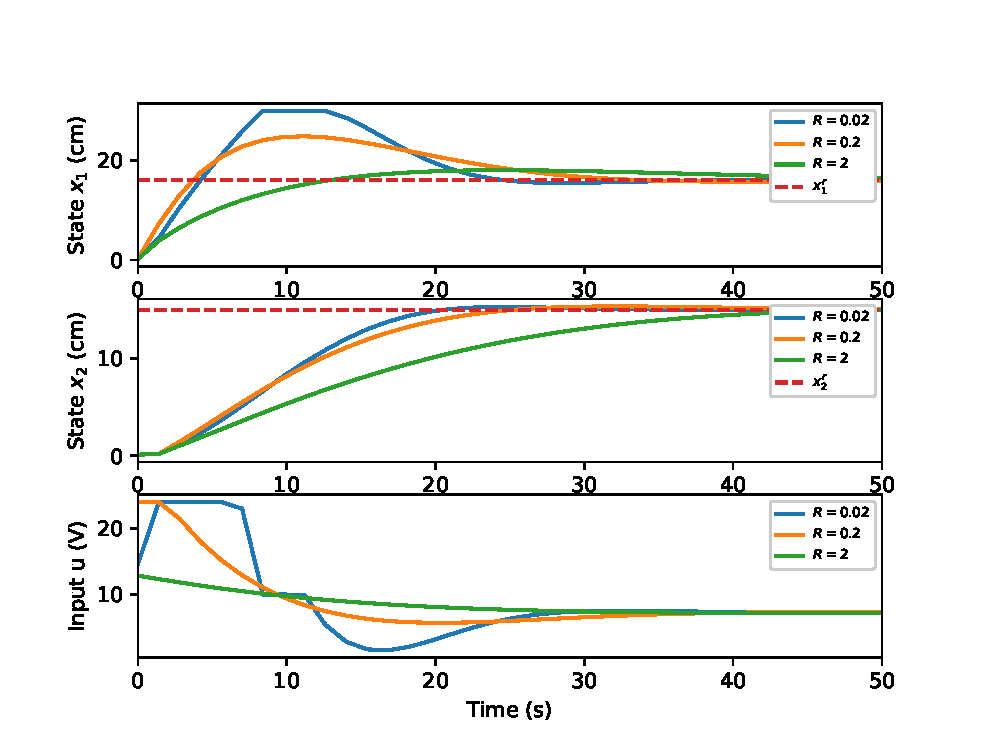
\includegraphics[width=0.45\textwidth]{img/tmpc2.eps} %{<left> <lower> <right> <upper>}
    \caption{Influence of input penalty $R$ on the closed-loop response.}
    \label{fig:tmpc2}
\end{figure}

\begin{figure}[h]
    \centering
    \includegraphics[width=0.45\textwidth]{img/tmpc3.eps} %{<left> <lower> <right> <upper>}
    \caption{Evolution of the objective value at first iteration, $J^{1,n}$.}
    \label{fig:tmpc3}
\end{figure}

\begin{figure}[h]
    \centering
    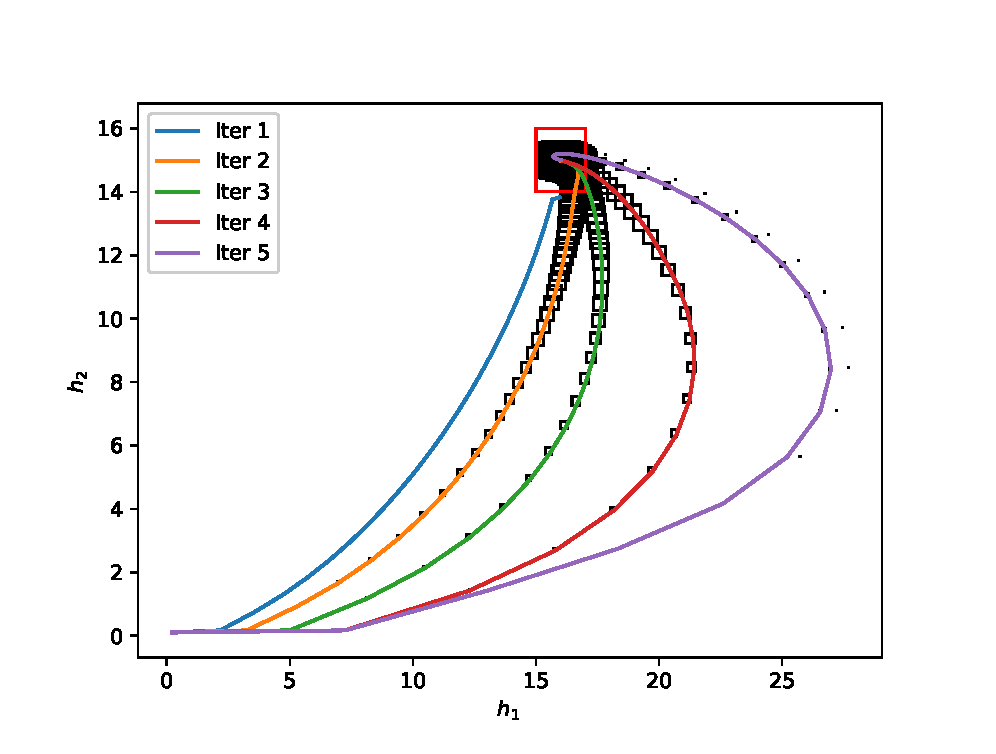
\includegraphics[width=0.45\textwidth]{img/tmpc4.eps} %{<left> <lower> <right> <upper>}
    \caption{Phase portrait at time step $n=0$ with successive predicted state trajectories, associated bounds (black boxes) and terminal set (red box).}
    \label{fig:tmpc4}
\end{figure}


We now compare the convergence properties of DC-TMPC with the successive linearisation tube-based MPC algorithm in \cite{mark} (MPC-2011). As described in Section~\ref{sec:TMPC}, linearisation errors around predicted trajectories are treated as disturbances in MPC-2011. The approach uses state- and control-dependent bounds on these errors, but these are determined assuming a fixed operating region. Hence the approach is more conservative than DC-TMPC, which exploits the convex nature of the linearisation errors to find tighter bounds on the state perturbations. As a result, it is expected that DC-TMPC demonstrates faster convergence and a larger set of feasible initial conditions than MPC-2011. To demonstrate this, we apply the MPC-2011 algorithm to the coupled tanks model with the same parameters. 
For a given terminal set, the range of open loop input voltage allowable for initialising the algorithm with a feasible problem was found to be $[6.1, 9.3]$~V for DC-TMPC, while it was limited between $[7.2, 7.8]$ V for MPC-2011, showing a smaller feasible initial conditions set. This demonstrates the relative conservativeness of the state perturbation bounds in MPC-2011 over DC-TMPC, as expected. Finally, the faster convergence of DC-TMPC is shown in Figure \ref{fig:tmpc5}, which compares the evolution of the objective value for both algorithms at the first time step, $J^{j,0}$, $j=1,\ldots,5$. This achieves to demonstrate the superiority of DC-TMPC over the tube-based MPC-2011 algorithm with successive linearisations.  

\begin{figure}[h]
    \centering
    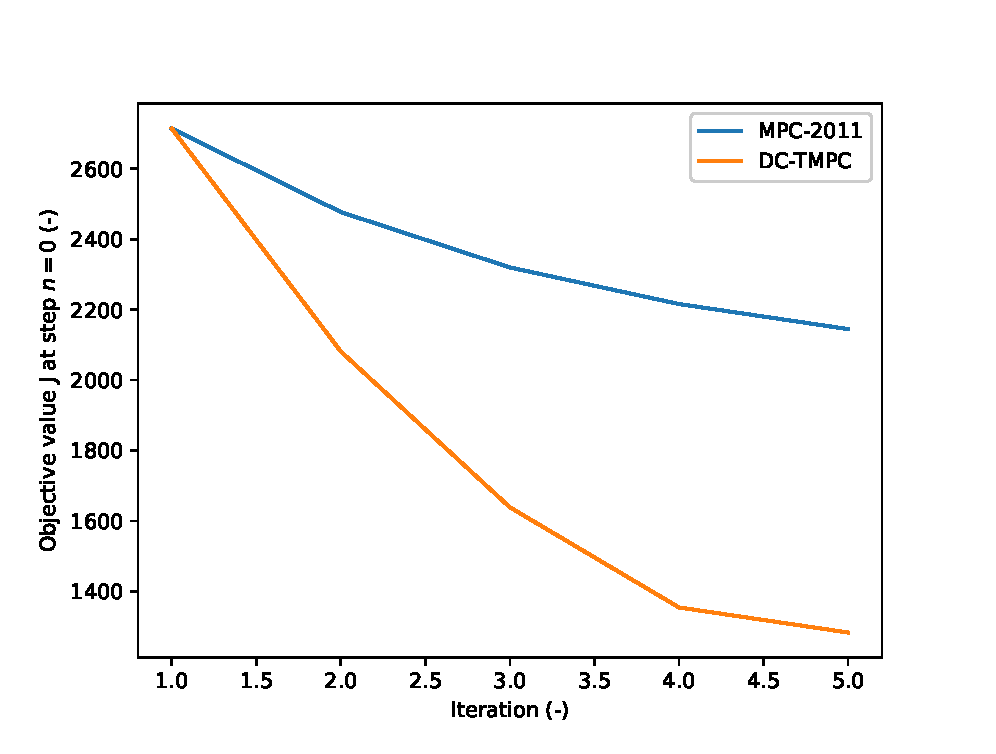
\includegraphics[width=0.45\textwidth]{img/tmpc5.eps} %{<left> <lower> <right> <upper>}
    \caption{Comparison of the objective value $J^{j,0}$ for both algorithms.}
    \label{fig:tmpc5}
\end{figure}

\section{Conclusion}
\label{sec:conclusion}

This paper introduces DC-TMPC, a new method for robust nonlinear MPC applied to systems representable as a difference of convex functions. The method relies on successively approximating the system dynamics around predicted trajectories and exploits convexity in the linearisation errors to construct robust and non-conservative tubes containing the perturbed trajectories. Convergence, recursive feasibility and asymptotic stability of the proposed algorithm are demonstrated. The algorithm is applied to regulation of fluid levels in a coupled tank system. 

Future work will include generalisation of the method to robustly stabilise the system in the presence of (additive) external disturbances, use of other parameterisations of the tube (e.g. ellipsoids or more general polytopes), and applications to problems such as robust trajectory generation for VTOL aircraft.
%applications to other systems representable as a difference of convex functions (e.g. the Fermi-Pasta-Ulam oscillator) and inclusion of the state feedback matrix $K_k$  in the optimisation to control the size of the tube online.  

%Another extension would be to investigate the application of DC-TMPC to a broader class of systems whose dynamics are two-times continuously differentiable. Indeed, $C^2$ functions can be decomposed as a difference of convex functions and the DC-TMPC paradigm could be applied. This requires to find a DC decomposition that  minimises conservativeness of the generated tube, which might prove challenging. In particular, functions that admit a piecewise definition in terms of convex and concave functions (e.g. $f(x) = x^3$ or the restriction of $f(x) = \sin(x)$ to the interval $x \in [-\pi/2, \pi/2]$) can be naturally decomposed as a difference of convex functions for which the DC-TMPC algorithm could be applied. 

\bibliography{biblio} 
\bibliographystyle{ieeetr}

\appendix
We summarise here a method for computing the terminal gain $\hat{K}$, terminal weighting matrix $\hat{Q}$, and terminal set bound $\hat{\gamma}$ by solving a semidefinite program (SDP).
%
Given bounds $\bar{\X}=\{x : \lvert x - x^r \rvert \leq \delta^x\}\subseteq\X$, $\bar{\U} = \{u: \lvert u - u^r \rvert \leq \delta^u\}\subseteq\U$ on the state and control input within the terminal set, we assume that the nonlinear system dynamics 
can be represented in $\bar{\X}\times\bar{\U}$
%locally near $(x^r,u^r)$ 
using a set of linear models.
The model approximation is assumed to satisfy, for all $k$,
\begin{equation}\label{eq:ldi_approx}
\begin{aligned}
f(x,u) - f(x^r, u^r) &\in \Co\{ A^{(i)} (x-x^r_k) + B^{(i)} (u - u^r_k), 
\\
&\qquad \quad i = 1,\ldots,m\} , \ \forall (x,u) \in \bar{\X}\times \bar{\U}
\end{aligned}
\end{equation}
(where $\Co$ denotes the convex hull). 
In order that $\hat{Q}$ and $\hat{K}$ satisfy the inequality (\ref{eq:Q_N}) we require, for all $ x\in \bar{\X}$,
\begin{align*}
\|x - x^r \|^2_{\hat{Q}} &\geq \bigl\|A^{(i)} (x-x^r) + B^{(i)} \hat{K} (x -x^r) \bigr\|^2_{\hat{Q}}  
\\
&\quad + \|x-x^r\|^2_Q + \|\hat{K} (x-x^r) \|^2_R .
%\ \forall x\in \bar{\X}.
%\label{eq:term_weight_quad}
\end{align*}
Since each term is quadratic in $x-x^r$, this condition is equivalent to a set of matrix inequalities, for $i = 1,\ldots,m$,
\[%\begin{align*}
\hat{Q} \succeq (A^{(i)}+B^{(i)}\hat{K})^\top \hat{Q} (A^{(i)}+B^{(i)}\hat{K}) + Q + \hat{K}^\top R \hat{K} ,
\]%\end{align*}
which can be expressed equivalently using Schur complements as LMIs in variables $S = \hat{Q}^{-1}$ and $Y = \hat{K}\hat{Q}^{-1}$:
\begin{equation}\label{eq:term_weight_lmi}
\begin{bmatrix}
S & (A^{(i)}S + B^{(i)}Y)^\top & S & Y \\
\star & S & 0 & 0 \\
\star & \star & Q^{-1} & 0 \\
\star & \star & \star &  R^{-1} 
\end{bmatrix} \succeq 0, \ i = 1,\ldots,m.
\end{equation}
To ensure that the model approximation (\ref{eq:ldi_approx}) remains valid we can exploit the positive invariance of the set $\hat{\X}=\{x : \|x - x^r\|_{\hat{Q}} \leq \hat{\gamma}\}$ for all $\hat{\gamma} > 0$, 
%that is implied by (\ref{eq:Q_N}) 
and impose the constraints
\[
\{x : \|x-x^r\|_{\hat{Q}}^2 \leq \hat{\gamma}\} \subseteq \bar{\X} \cap \{ x: Kx \in \bar{\U}\} 
\]
which are equivalent to
\begin{align}
\hat{\gamma}^{-1} [ \delta^x ]_i^2 - [S]_{ii} \succeq 0, &  &i = 1,\ldots,n_x
\label{eq:termxcon}\\
\begin{bmatrix} \hat{\gamma}^{-1}[\delta^u ]_i^2 & [Y]_i \\ \star & S \end{bmatrix} \succeq 0, & & i = 1,\ldots,n_u
\label{eq:termucon}
\end{align}
To balance the requirements for good terminal controller performance and a large terminal set, we can minimise $\tr(\hat{Q}) + \alpha \hat{\gamma}^{-1}$ subject to the constraints (\ref{eq:term_weight_lmi}), (\ref{eq:termxcon}), (\ref{eq:termucon}) and
\begin{equation}\label{eq:Sbnd}
\begin{bmatrix} S & I \\ \star & \hat{Q} \end{bmatrix} \succ 0 ,
\end{equation}
over variables $S=S^\top$, $Y$ and $\hat{\gamma}^{-1}$, where $\alpha$ is a scalar constant that controls the trade-off between the competing objectives of minimising $\tr(\hat{Q})$ and minimising $\hat{\gamma}^{-1}$.

%provides $\hat{Q}$ and $\hat{K}$ satisfying (\ref{eq:Q_N}). 
%associated to state and input square terminal sets of respective side length $2\delta^x$ and  $2\delta^u$. 
%and where $K_N = YQ_N$.

\end{document}
 